\documentclass[tikz,border=4pt]{standalone}
% Shared visual grammar: role fills, dark connectors, and 7-point typography.
% Build each standalone figure from this directory. No external images required.
\pdfinfoomitdate=1
\pdftrailerid{}
\usepackage[T1]{fontenc}
\usepackage{helvet}
\renewcommand{\familydefault}{\sfdefault}
\usepackage{amsmath,amssymb}
\hyphenpenalty=10000
\exhyphenpenalty=10000
\usetikzlibrary{arrows.meta,calc,fit,positioning,decorations.pathreplacing,backgrounds}
\definecolor{ink}{HTML}{172B3A}
\definecolor{muted}{HTML}{586D85}
\definecolor{datafill}{HTML}{F1F5F9}
\definecolor{dataline}{HTML}{62748E}
\definecolor{modelfill}{HTML}{E5E9FF}
\definecolor{modelline}{HTML}{7887C7}
\definecolor{llmfill}{HTML}{FFE4E8}
\definecolor{llmline}{HTML}{E68494}
\definecolor{truthfill}{HTML}{D0FAE5}
\definecolor{truthline}{HTML}{35A782}
\newcommand{\seven}{\fontsize{7}{8.5}\selectfont}
\tikzset{
 every node/.append style={font=\seven,text=ink,align=center},
 box/.style={draw=dataline,fill=white,rounded corners=3pt,line width=.65pt,inner sep=5pt,minimum height=8mm},
 data/.style={box,fill=datafill},
 model/.style={box,draw=modelline,fill=modelfill},
 llm/.style={box,draw=llmline,fill=llmfill},
 truth/.style={box,draw=truthline,fill=truthfill},
 title/.style={font=\seven\bfseries,inner sep=1pt},
 word/.style={text=muted,inner sep=1pt,align=center},
 label/.style={fill=white,inner xsep=2pt,inner ysep=1pt,text=muted},
 flow/.style={-{Stealth[length=2.4mm,width=1.9mm]},draw=ink,line width=1.2pt,shorten >=1.5pt},
 branch/.style={-{Stealth[length=2mm,width=1.6mm]},draw=ink,line width=.9pt,shorten >=1pt},
 route/.style={draw=ink,line width=1.2pt},
 update/.style={-{Stealth[length=2.2mm,width=1.7mm]},draw=modelline,line width=1pt,dash pattern=on 3pt off 2pt,shorten >=1.5pt},
 boundary/.style={draw=dataline,dash pattern=on 3pt off 2pt,rounded corners=3pt,line width=.6pt},
 chip/.style={minimum height=4mm,inner xsep=3pt,inner ysep=1.5pt,rounded corners=2pt},
}
% Optional role key. Anchor at the center of an uncluttered final row.
\newcommand{\rolekey}[2]{
 \node[word,anchor=east] at (#1-6.6,#2) {\textit{Key}};
 \node[data,chip] at (#1-5.2,#2) {records / data};
 \node[model,chip] at (#1-1.9,#2) {learned model / policy};
 \node[llm,chip] at (#1+1.65,#2) {LLM signal};
 \node[truth,chip] at (#1+4.95,#2) {labels / evaluation};
}

\newcommand{\nine}{\fontsize{9}{11.3}\selectfont}
\newcommand{\eight}{\fontsize{8}{10}\selectfont}
\begin{document}
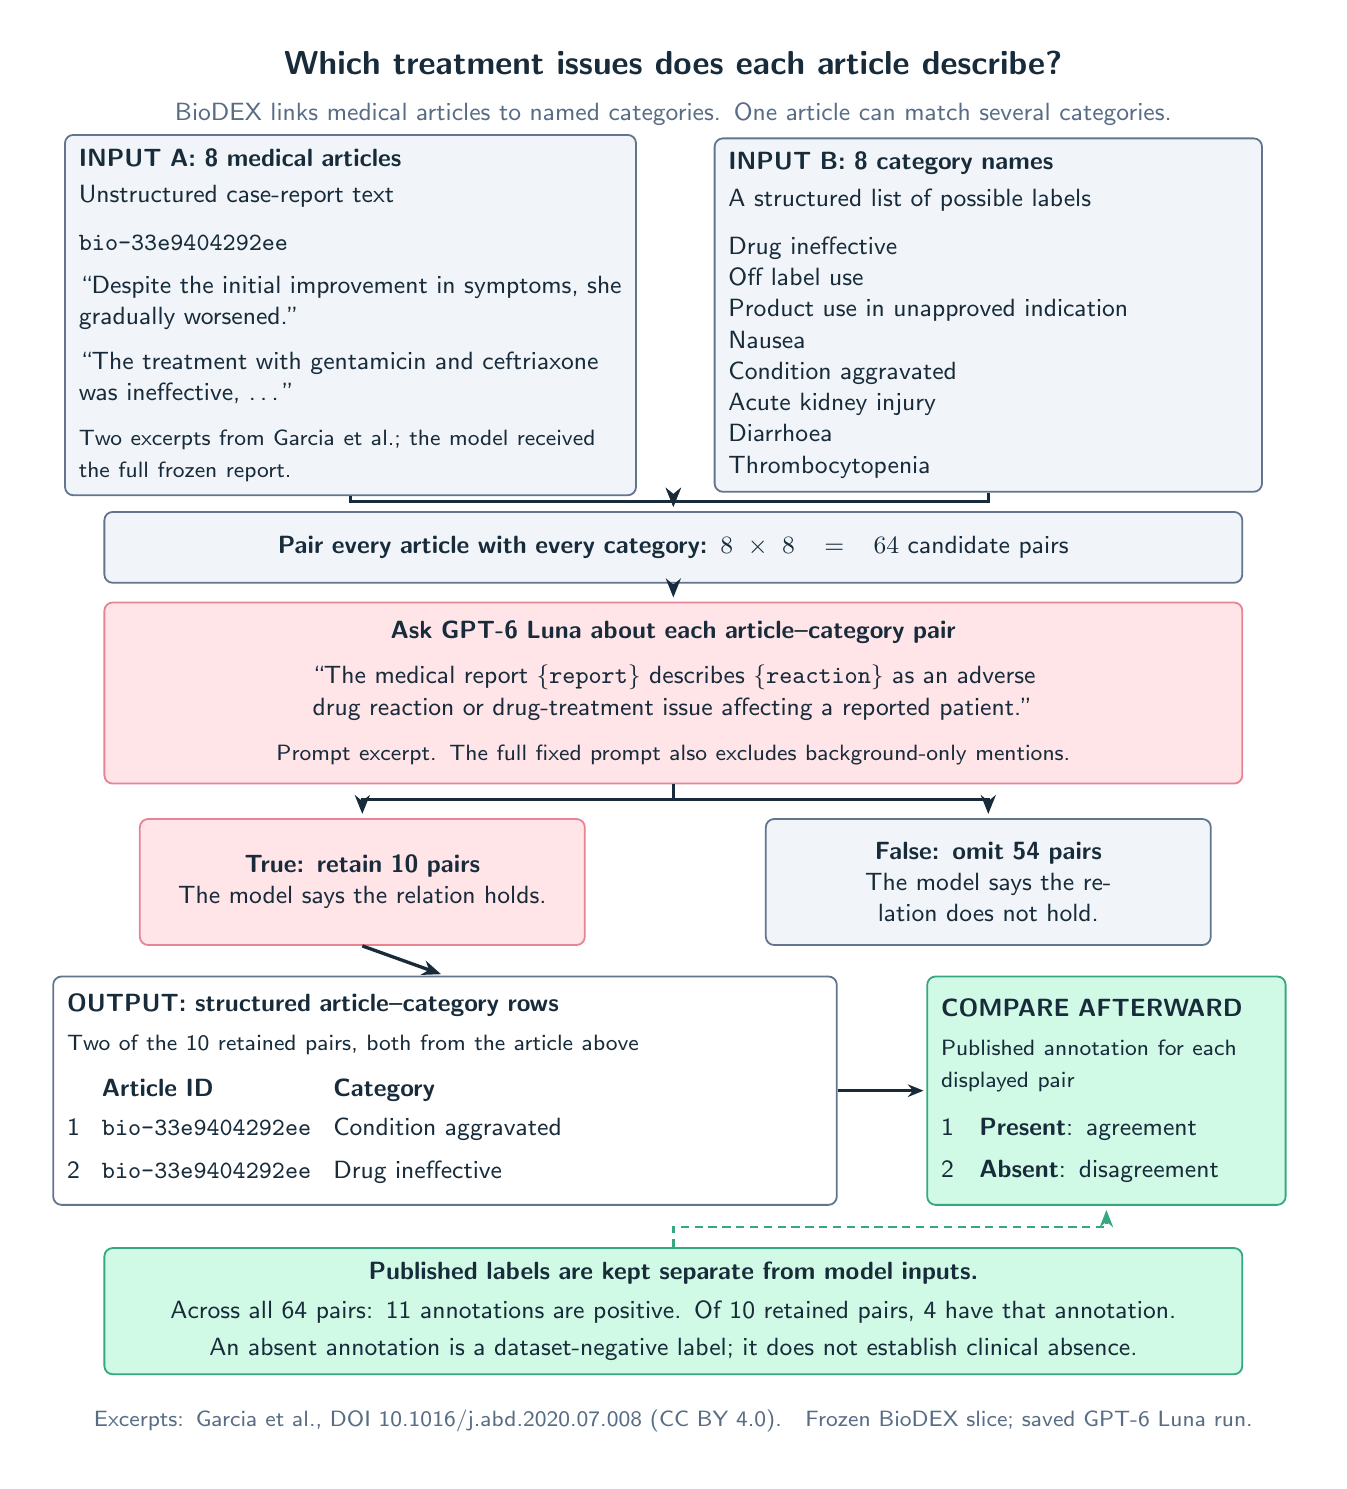
\begin{tikzpicture}[every node/.append style={font=\nine}]
\useasboundingbox (-.2,.3) rectangle (16.2,-17.9);

\node[font=\fontsize{12}{14}\selectfont\bfseries,text width=155mm] at (8,-.15)
  {Which treatment issues does each article describe?};
\node[word,font=\nine,text width=150mm] at (8,-.8)
  {BioDEX links medical articles to named categories. One article can match several categories.};

\node[data,text width=69mm,minimum height=43mm,align=left] (articles) at (3.9,-3.35) {
  \textbf{INPUT A: 8 medical articles}\\[2pt]
  Unstructured case-report text\\[6pt]
  \texttt{bio-33e9404292ee}\\[4pt]
  ``Despite the initial improvement in symptoms, she gradually worsened.''\\[5pt]
  ``The treatment with gentamicin and ceftriaxone was ineffective, \ldots''\\[5pt]
  {\eight Two excerpts from Garcia et al.; the model received the full frozen report.}
};

\node[data,text width=66mm,minimum height=43mm,align=left] (categories) at (12,-3.35) {
  \textbf{INPUT B: 8 category names}\\[2pt]
  A structured list of possible labels\\[6pt]
  Drug ineffective\\
  Off label use\\
  Product use in unapproved indication\\
  Nausea\\
  Condition aggravated\\
  Acute kidney injury\\
  Diarrhoea\\
  Thrombocytopenia
};

\node[data,text width=141mm,minimum height=9mm] (pairs) at (8,-6.3)
  {\textbf{Pair every article with every category:} $8\times8=64$ candidate pairs};
\draw[flow] (articles.south) -- (3.9,-5.72) -| (pairs.north);
\draw[flow] (categories.south) -- (12,-5.72) -| (pairs.north);

\node[llm,text width=141mm,minimum height=23mm] (llm) at (8,-8.15) {
  \textbf{Ask GPT-6 Luna about each article--category pair}\\[5pt]
  ``The medical report \texttt{\{report\}} describes \texttt{\{reaction\}} as an adverse drug reaction
  or drug-treatment issue affecting a reported patient.''\\[5pt]
  {\eight Prompt excerpt. The full fixed prompt also excludes background-only mentions.}
};
\draw[flow] (pairs.south) -- (llm.north);

\node[llm,text width=53mm,minimum height=16mm] (yes) at (4.05,-10.55)
  {\textbf{True: retain 10 pairs}\\The model says the relation holds.};
\node[data,text width=53mm,minimum height=16mm] (no) at (12,-10.55)
  {\textbf{False: omit 54 pairs}\\The model says the relation does not hold.};
\draw[flow] (llm.south) -- (8,-9.5) -| (yes.north);
\draw[flow] (8,-9.5) -| (no.north);

\node[box,text width=96mm,minimum height=29mm,align=left] (output) at (5.1,-13.2) {
  \textbf{OUTPUT: structured article--category rows}\\[3pt]
  {\eight Two of the 10 retained pairs, both from the article above}\\[6pt]
  \setlength{\tabcolsep}{4pt}
  \begin{tabular}{@{}rll@{}}
   & \textbf{Article ID} & \textbf{Category}\\[3pt]
  1 & \texttt{bio-33e9404292ee} & Condition aggravated\\[4pt]
  2 & \texttt{bio-33e9404292ee} & Drug ineffective
  \end{tabular}
};
\draw[flow] (yes.south) -- (output.north);

\node[truth,text width=42mm,minimum height=29mm,align=left] (evaluation) at (13.5,-13.2) {
  \textbf{COMPARE AFTERWARD}\\[3pt]
  {\eight Published annotation for each displayed pair}\\[6pt]
  1\quad\textbf{Present}: agreement\\[4pt]
  2\quad\textbf{Absent}: disagreement
};
\draw[branch] (output.east) -- (evaluation.west);

\node[truth,text width=141mm,minimum height=15mm] (labels) at (8,-16.0) {
  \textbf{Published labels are kept separate from model inputs.}\\[3pt]
  Across all 64 pairs: 11 annotations are positive. Of 10 retained pairs, 4 have that annotation.\\[2pt]
  An absent annotation is a dataset-negative label; it does not establish clinical absence.
};
\draw[update,draw=truthline] (labels.north) -- (8,-14.93) -| (evaluation.south);

\node[word,font=\eight,text width=154mm] at (8,-17.4) {
  Excerpts: Garcia et al., DOI 10.1016/j.abd.2020.07.008 (CC BY 4.0).\quad
  Frozen BioDEX slice; saved GPT-6 Luna run.
};
\end{tikzpicture}
\end{document}
